\documentclass{article}%
\usepackage[T1]{fontenc}%
\usepackage[utf8]{inputenc}%
\usepackage{lmodern}%
\usepackage{textcomp}%
\usepackage{lastpage}%
\usepackage[head=40pt,margin=0.5in,bottom=0.6in]{geometry}%
\usepackage{graphicx}%
%
\title{\textbf{Jonidel Mendoza muestra en Madrid la sólida transparencia de su humanidad}}%
\author{JUAN ANTONIO GONZÁLEZ}%
\date{04/03/2019}%
%
\begin{document}%
\normalsize%
\maketitle%
\textbf{URL: }%
http://www.eluniversal.com/entretenimiento/34689/jonidel{-}mendoza{-}muestra{-}en{-}madrid{-}la{-}solida{-}transparencia{-}de{-}su{-}humanidad\newline%
%
\textbf{Periodico: }%
EU, %
ID: %
34689, %
Seccion: %
entretenimiento\newline%
%
\textbf{Palabras Claves: }%
NO\_TIENE\newline%
%
\textbf{Derecho: }%
2.1%
, Otros Derechos: %
\newline%
%
\textbf{\textit{El artista venezolano inaugura hoy en la galería madrileña In Casa, y en alianza con la venezolana GBG Arts, la exposición “Encuentros/Desencuentros”}}%
\newline%
\newline%
%
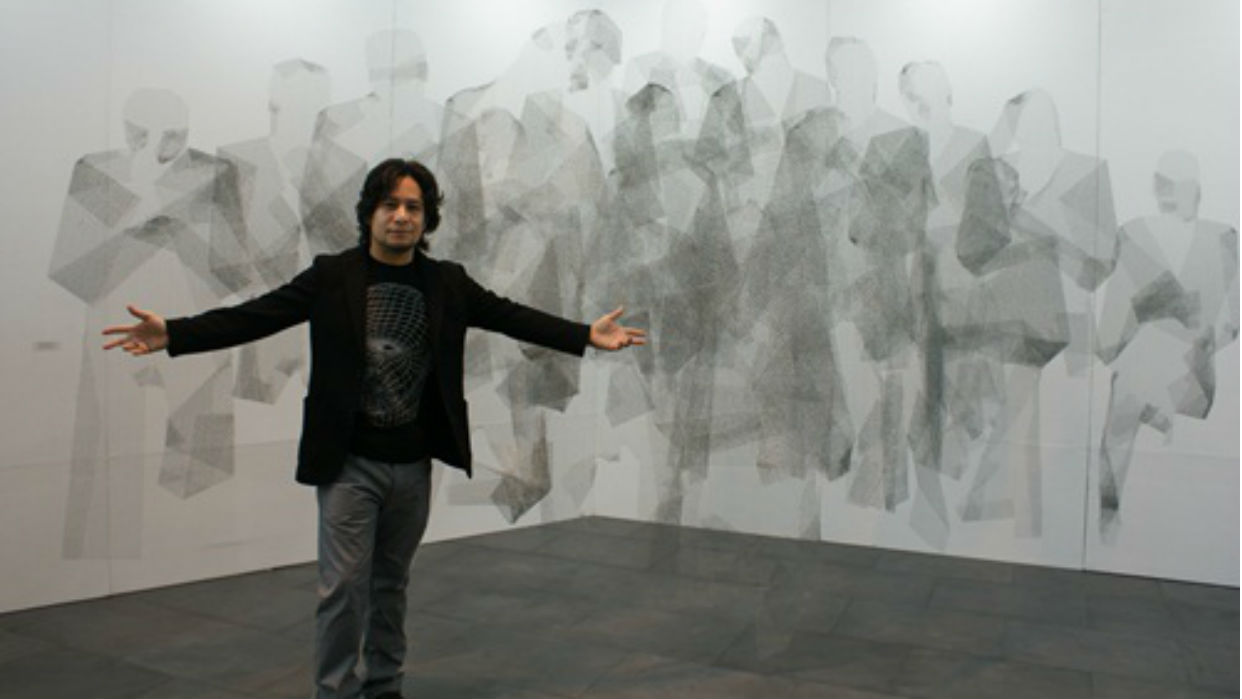
\includegraphics[width=300px]{EU_34689.jpg}%
\newline%
%
La obra del artista venezolano Jonidel Mendoza (Maturín, estado Monagas, 1975) es un permanente juego de revelaciones y ocultamientos, de apariciones y desapariciones, de%
\newline%
%
, título este de la exposición que se inaugura hoy en la galería In Casa, ubicada en la calle de Villanueva 5, 28001, de Madrid, en alianza con su par venezolana GBG Arts.%
\newline%
%
En la muestra, que permanecerá abierta hasta el 1° de abril, Mendoza presenta un cuerpo de trabajo en el que destaca el uso de técnicas y materiales diversos como el dibujo y la pintura y la fibra de vidrio, láminas de aluminio microperforadas, mallas metálicas, seda y organza, entre otros.Obras de la serie “Ecos del reflejo”El resultado de la investigación que realiza el artista, quien ha expuesto su obra, además de en Venezuela, en países como Estados Unidos, Corea del Sur, Colombia, Chile, Inglaterra, Francia y España, es una íntima reflexión sobre la fragilidad de la condición humana, sobre esas claves imprecisas que nos definen como individuos, como colectividad. Una humanidad que Jonidel Mendoza capta con iguales dosis de sutileza y violencia.Comenta Gabriela Benaim, directora de GBG Arts, que comenzó a trabajar con Mendoza en 2004. “Mario Matos y yo lo conocimos cuando era estudiante del Instituto Universitario de Estudios Superiores de Artes Plásticas Armando Reverón, en Caracas. Él formó parte de lo que la audiencia llamó ‘Los orientales’ y la primera exposición que hicimos fue la colectiva Pintón pasado pintura fresca, en la que estaban Starsky Brines, Paul Parrella, Enay Ferrer, José Vívenes y, por supuesto, Jonidel Mendoza. Nos fue increíble, creo que se vendió toda la exposición”, recuerda la galerista.“Todo lo hace él con sus propias manos, su trabajo es muy intimista. Trabaja las siluetas con alambres que luego son proyectadas a través de la iluminación. Sus seres son como una multitud, personas que comparten miradas, se ignoran, se encuentran y desencuentran”, agrega Benaim, que no duda en afirmar que Jonidel Mendoza es uno de los artistas más importantes de su generación.“The Translucentc Reflection”Encuentros/Desencuentros permitirá al público y a los coleccionistas españoles descubrir una propuesta que, como afirma la investigadora, crítico y docente de artes visuales María Elena Ramos, transmuta telas metálicas o fuertes mallas industriales en figuras ingrávidas. De acuerdo con la experta, el eje de las instalaciones de Mendoza son “entes tangibles y a la vez incorpóreos; apariencias de radiografías que recuerdan, del hombre, la constante convivencia –marcada por la realidad biológica– de lo exterior de su anatomía con la ósea estructura interna (...)”.Mendoza usa medios mixtos en sus propuestasEl curador e investigador Félix Suazo va más allá en su apreciación de las figuras inacabadas de Mendoza: “Son criaturas de apariencia evanescente, cual retratos de una existencia amenazada que se protege de incursiones indiscretas o perniciosas detrás de cercas, rejas y cortinas.  El  individuo {-}aislado o diluido en la multitud{-} es sólo una sugestión cuasi corpórea que lleva la marca del encierro”, escribe.%
\newline%
%
@juanchi62%
\newline%
%
\end{document}